{
\begin{figure}[th]
\begin{center}
\centerline{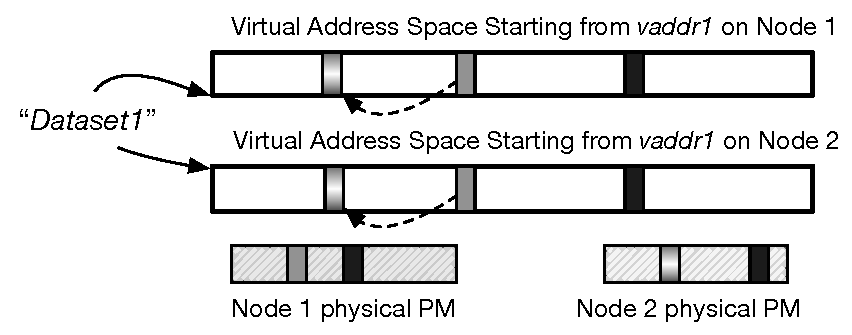
\includegraphics[width=\textwidth]{hotpot/Figures/addressing.pdf}}
\caption[\hotpot\ Addressing.]
{\hotpot\ Addressing.
\hotpot\ maps ``{\em Dataset1}'' to Node 1 and Node 2's virtual address space using the 
same base virtual addresses. The physical address mapping on each node is different.
The grey blocks in the middle are pointers that point to the blocks on the left. 
}
\label{fig-hotpot-addressing}
\end{center}
\end{figure}
}